\section{142 --- Linked List Cycle II}
Given a linked list with head node $H$, return the node where the cycle begins. If there is no cycle, return \texttt{null}.
\par
To represent a cycle in the given linked list, we use an integer $P$ which represents the position (0-indexed) in the linked list where tail connects to. If $P$ is $-1$, then there is no cycle in the linked list.
\par
\textbf{Note}: Do not modify the linked list.
\paragraph{Example 1:}
\begin{flushleft}
\textbf{Input}:$P = 1$, $L$ is shown as below
\begin{figure}[H]
\begin{tikzpicture}
[mynode/.style={draw,circle,minimum size=8mm, fill=gray!20!}]
\node(){};
\node[mynode](3) {3};
\node[mynode](2)[right=15mm of 3] {2};
\node[mynode](0)[right=15mm of 2] {0};
\node[mynode](M4)[right=15mm of 0] {-4};
\draw[>=stealth,->] (3) -- (2);
\draw[>=stealth,->] (2) -- (0);
\draw[>=stealth,->] (0) -- (M4);
\draw[>=stealth,->] (M4) to[bend left=45] (2);
\end{tikzpicture}
\end{figure}
\textbf{Output}: tail connects to node index 1
\\
\textbf{Explanation}: There is a cycle in the linked list, where tail connects to the second node.
\end{flushleft}
\paragraph{Example 2:}
\begin{flushleft}
\textbf{Input}: $P=0$, $L$ is shown as below
\begin{figure}[H]
\begin{tikzpicture}
[mynode/.style={draw,circle,minimum size=8mm, fill=gray!20!}]
\node(){};
\node[mynode](1) {1};
\node[mynode](2)[right=15mm of 1] {2};
\draw[>=stealth,->] (1) -- (2);
\draw[>=stealth,->] (2) to[bend left=45] (1);
\end{tikzpicture}
\end{figure}
\textbf{Output}: tail connects to node index 0
\\
\textbf{Explanation}: There is a cycle in the linked list, where tail connects to the first node.
\end{flushleft}
\paragraph{Example 3:}
\begin{flushleft}
\textbf{Input}: $P=-1$, $L$ is
\begin{figure}[H]
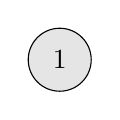
\begin{tikzpicture}
[mynode/.style={draw,circle,minimum size=8mm, fill=gray!20!}]
\node(){};
\node[mynode](1) {1};
\end{tikzpicture}
\end{figure}
\textbf{Output}: no cycle
\\
\textbf{Explanation}: There is no cycle in the linked list.
\end{flushleft}
\paragraph{Follow up:}
\begin{itemize}
\item Can you solve it without using extra space?
\end{itemize}
\subsection{Two Pointers}
首先还是用快慢指针确定是否是存在circle的linked list。如果是,则在两个指针相遇处,将另外一个指针重新指向list的header,然后两个指针每次都只前进一步,直至相遇,这时候的相遇处就是cycle begin的位置。
\setcounter{algorithm}{0}
\begin{algorithm}[H]
\caption{Two Pointers}
\begin{algorithmic}[1]
\Procedure{DetectCycle}{$H$}
\If{$H=\texttt{null}$}
\State \Return \texttt{false} \Comment Empty list
\EndIf
\State $F:=H$ \Comment The fast pointer
\State $S:=H$ \Comment The slow pointer
\State $b:=\texttt{false}$ \Comment The boolean variable indicate if there is a cycle
\While{$F\neq \texttt{null}$ \textbf{and} $F.\texttt{next}\neq \texttt{null}$} \label{142while}
\State $F\gets F.\texttt{next}$
\State $F\gets F.\texttt{next}$ \Comment $F$ move forward two steps
\State $S\gets S.\texttt{next}$ \Comment $S$ move forward one step
\If{$F=S$}
\State $b\gets \texttt{true}$
\State \texttt{break} \Comment End[\ref{142while}]
\EndIf
\EndWhile
\If{$b=\texttt{false}$}
\State \Return \texttt{null} \Comment No cicle in the list
\EndIf
\State $F\gets H$ \Comment Reset $F$ to header node
\While{$F\neq S$}
\State $F\gets F.\texttt{next}$ \Comment $F$ move forward one step
\State $S\gets S.\texttt{next}$ \Comment $S$ move forward one step
\EndWhile
\State \Return $S$ or $F$ \Comment $S$ and $F$ are met at the start of circle
\EndProcedure
\end{algorithmic}
\end{algorithm}